\setlength{\parindent}{0em}

\chapter{Resultados}\label{cap4}\thispagestyle{fancy}

\vspace{-1.3cm}

\section{Resultados}

Como se han mencionado en cápitulos anteriores el resultado de las pruebas ha sido positivo

En la gráfica siguiente se muestra cómo va evolucionando el capital de la cuenta simulada, se puede observar todas las predicciones que realizan los
modelos y el sharpe ratio final.

\begin{figure}[h]
    \centering
    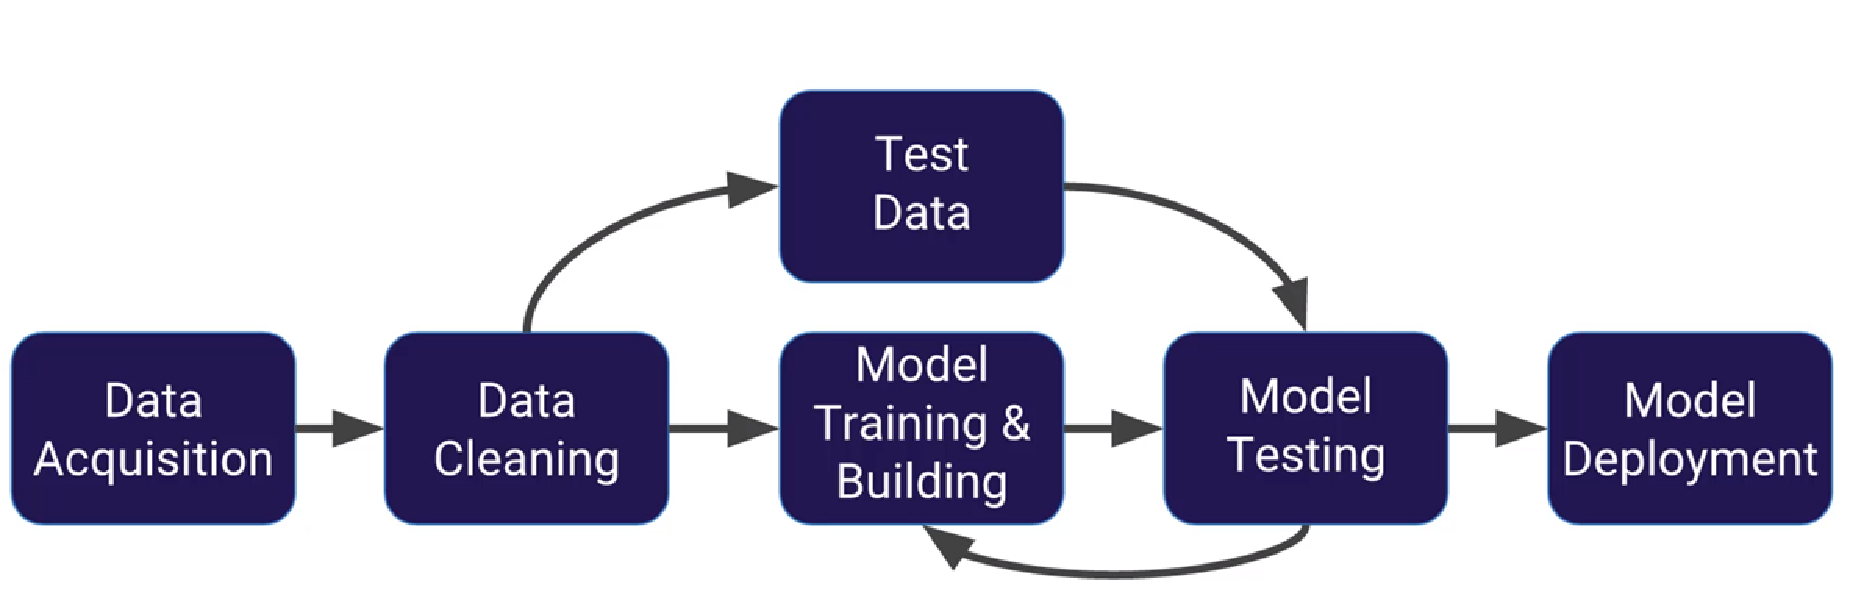
\includegraphics[scale=0.45]{./img/ml_process.pdf}
    \caption{Añadir img con equity curve, max drawdown y sharpe ratio}
    \label{fig_mlp_6}
\end{figure}

Para poner en perspectiva los resultados he decidido compararlos con los obtenidos por los participantes de la competición Robotrader, competición en
la cuál iba a participar en un inicio pero que por imcopatibilidad con el desarrollo de este proyecto no acabé participando. Como se puede observar la
curva mejora a muchos de los sistemas presentados.

La competición se realizó durante los meses de marzo a mayo, estos datos nunca se han usado para entrenar los modelos para evitar leakage. No es una
comparación perfecta ya que no se tienen en cuenta todos los problemas que pueden haber en vivo pero se han intentado simular lo mejor posible.

\begin{figure}[h]
    \centering
    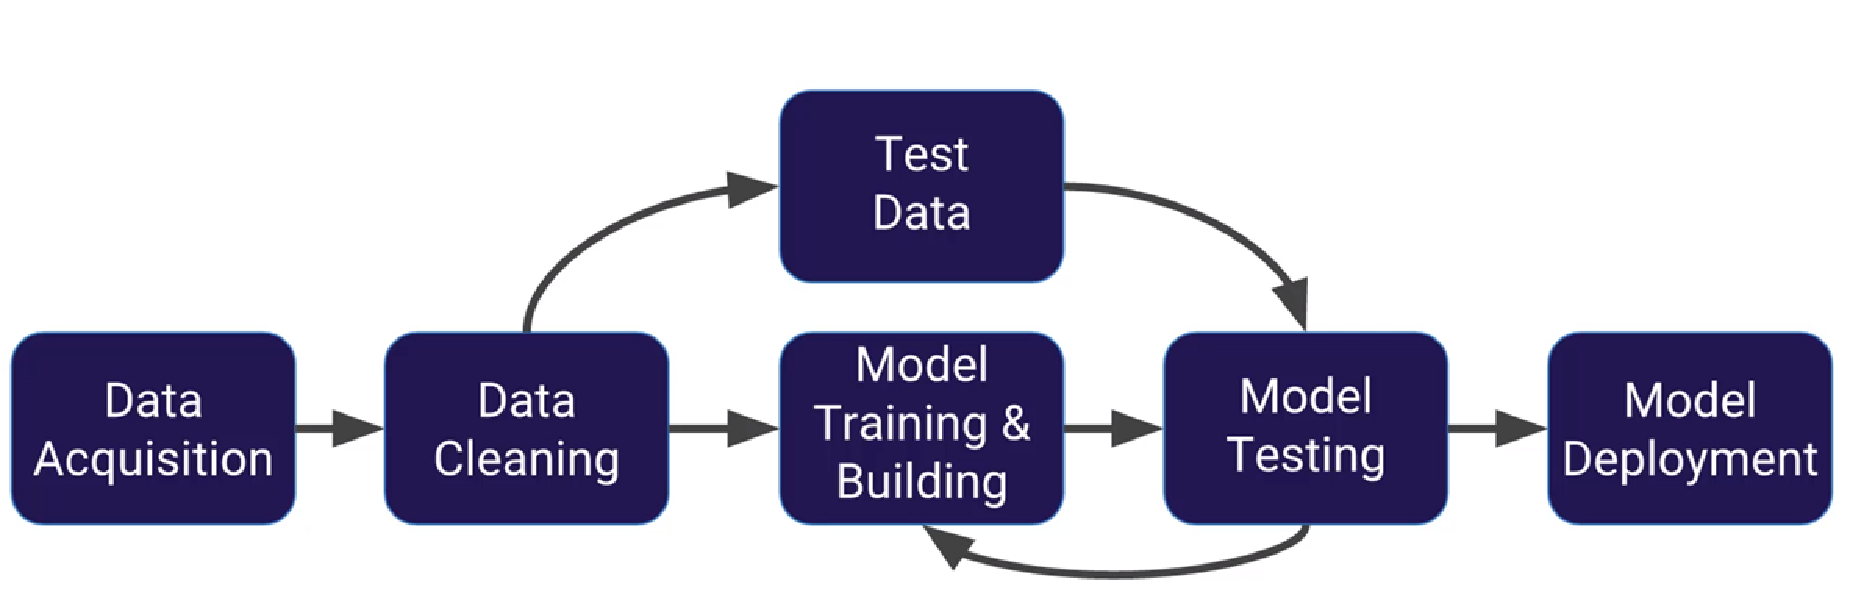
\includegraphics[scale=0.45]{./img/ml_process.pdf}
    \caption{Añadir img comparativa del Backtest vs Robotrader}
    \label{fig_mlp_13}
\end{figure}

Además de mostrar los datos teóricos que se hubiesen conseguido también he querido comparar con los datos de la simulación de Monte Carlo.

\begin{figure}[h]
    \centering
    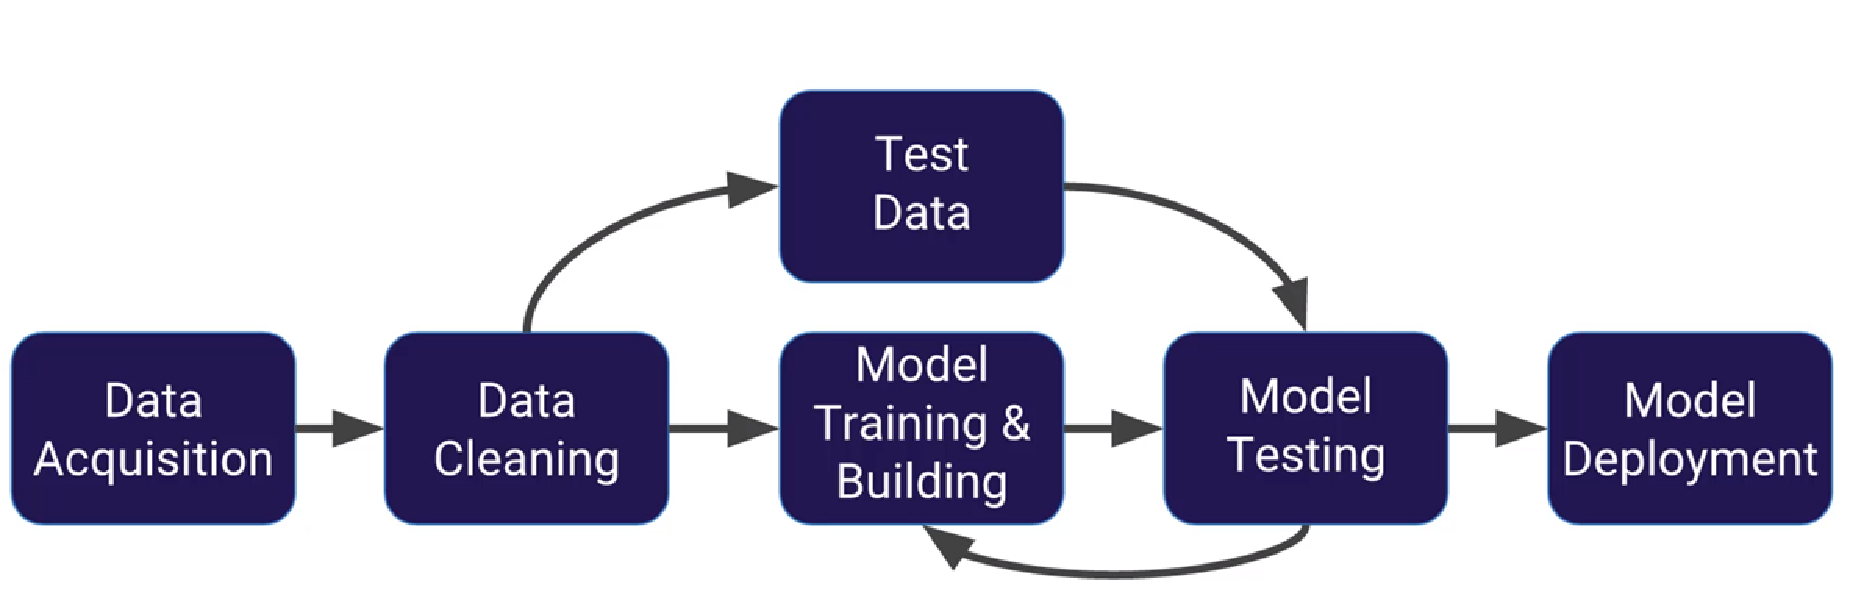
\includegraphics[scale=0.45]{./img/ml_process.pdf}
    \caption{Añadir img comparativa del Monte Carlo vs Robotrader}
    \label{fig_mlp_14}
\end{figure}

\begin{figure}[H]
    \centering
    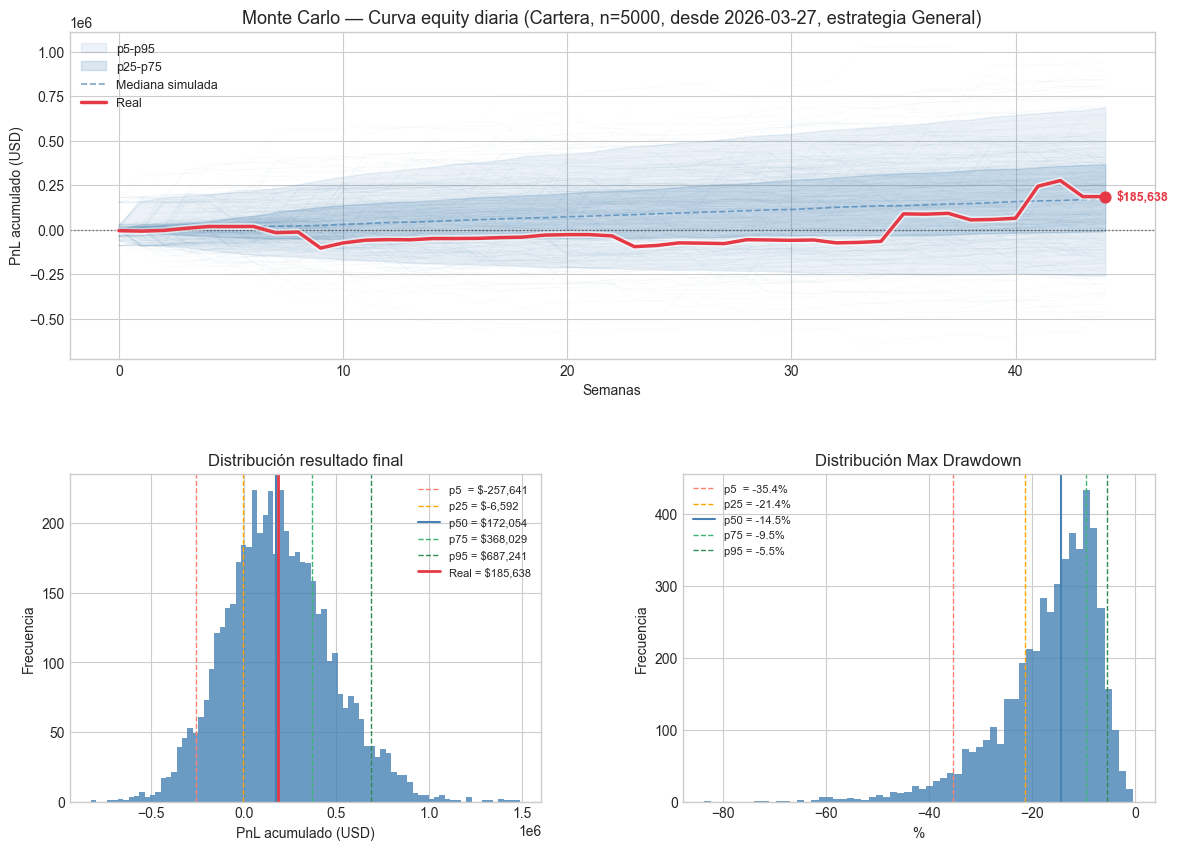
\includegraphics[width=\textwidth]{./img/monte_carlo_mal.png}
    \caption{Añadir img comparativa del Monte Carlo vs Robotrader}
    \label{fig_mlp_24}
\end{figure}

\begin{figure}[H]
    \centering
    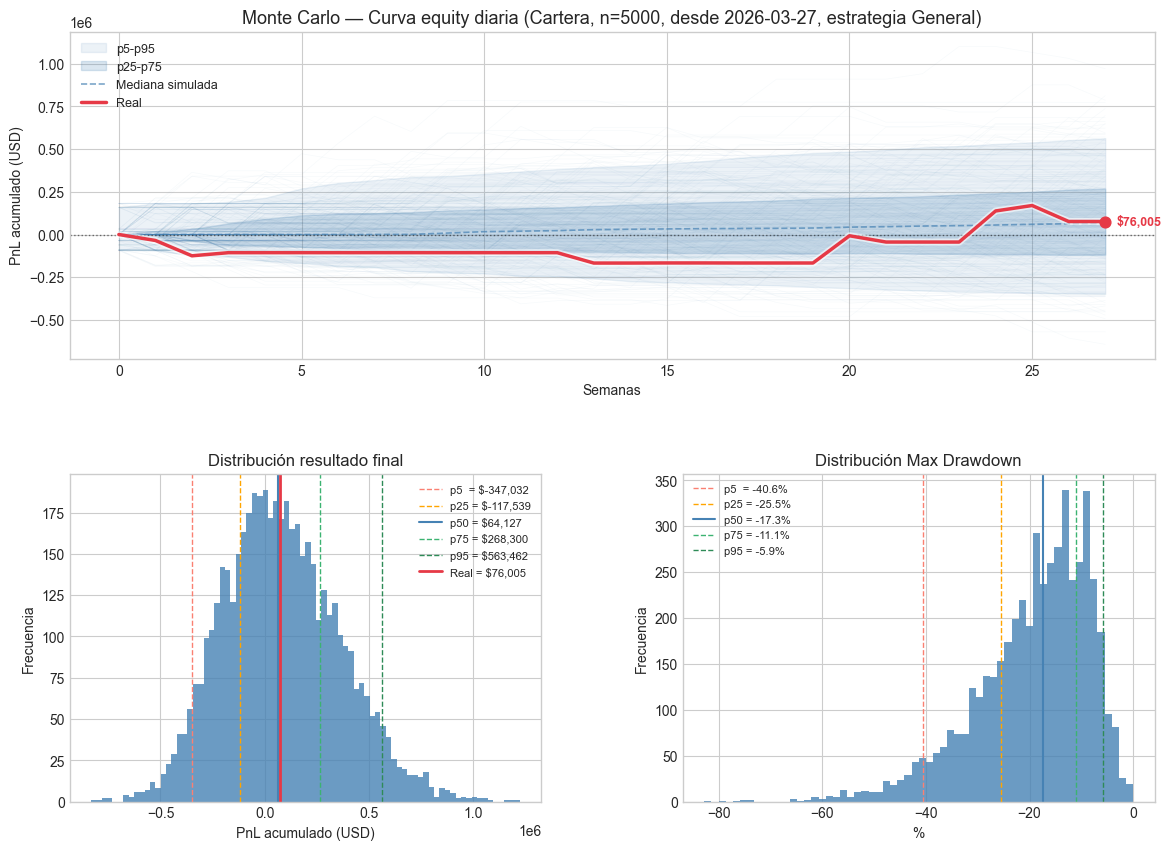
\includegraphics[width=\textwidth]{./img/monte_carlo_bien.png}
    \caption{Añadir img comparativa del Monte Carlo vs Robotrader}
    \label{fig_mlp_25}
\end{figure}

\notes{Añadir grafica de la evolución del equity, comparativa contra Robotrader} 

\notes{Añadir Monte Carlo}

\begin{table}[H]
\centering
\makebox[0pt]{%
\begin{tabular}{|c|c|c|c|c|c|c|}
\hline
\multirow{2}{*}{\textbf{Futuro}} &
\multirow{2}{*}{\textbf{Capital inicial}} &
\multicolumn{4}{c|}{\textbf{Capital final}} &
\multirow{2}{*}{\textbf{Ganancias mejor caso}} \\ \cline{3-6}
 & & \textbf{Normal} & \textbf{Scale-in} & \textbf{Sizing} & \textbf{Scale-in + Sizing} & \\ \hline

AD   & 30k  & \multicolumn{4}{c|}{No hay operaciones}                                                        & 0 \\ \hline
BP   & 30k  & \multicolumn{4}{c|}{Por alguna razón faltan dos features}                                      & 0 \\ \hline
CL   & 300k & \multicolumn{1}{c|}{305k}  & \multicolumn{1}{c|}{317k}   & \multicolumn{1}{c|}{306k}  & 400k   & \poscolor{100k} \\ \hline
EC   & 40k  & \multicolumn{4}{c|}{No hay operaciones}                                                        & 0 \\ \hline
ES   & 350k & \multicolumn{1}{c|}{320k}  & \multicolumn{1}{c|}{280k}   & \multicolumn{1}{c|}{349k}  & 250k   & \negcolor{-1k} \\ \hline
GC   & 450k & \multicolumn{1}{c|}{450k}  & \multicolumn{1}{c|}{465k}   & \multicolumn{1}{c|}{450k}  & 465k   & \poscolor{15k} \\ \hline
MFXI & 5k   & \multicolumn{1}{c|}{4.8k}  & \multicolumn{1}{c|}{4.75k}  & \multicolumn{1}{c|}{4.5k}  & 3.75k  & \negcolor{-0.2k} \\ \hline
NG   & 70k  & \multicolumn{1}{c|}{70k}   & \multicolumn{1}{c|}{69k}    & \multicolumn{1}{c|}{71k}   & 67k    & \poscolor{1k} \\ \hline
NQ   & 650k & \multicolumn{1}{c|}{630k}  & \multicolumn{1}{c|}{570k}   & \multicolumn{1}{c|}{650k}  & 550k   & 0 \\ \hline
YM   & 200k & \multicolumn{1}{c|}{198k}  & \multicolumn{1}{c|}{198k}   & \multicolumn{1}{c|}{200k}  & 196k   & 0 \\ \hline
ZB   & 50k  & \multicolumn{1}{c|}{50k}   & \multicolumn{1}{c|}{49k}    & \multicolumn{1}{c|}{50k}   & 48k    & 0 \\ \hline
ZN   & 30k  & \multicolumn{1}{c|}{25k}   & \multicolumn{1}{c|}{24k}    & \multicolumn{1}{c|}{22k}   & 0k     & \negcolor{-5k} \\ \hline
ZS   & 50k  & \multicolumn{1}{c|}{300k}  & \multicolumn{1}{c|}{300k}   & \multicolumn{1}{c|}{80k}   & 300k   & \poscolor{250k} \\ \hline

\end{tabular}

}
\caption{Tabla resumen de los 13 futuros evaluados en las cuatro modalidades operativas. Desde 2026-01-20 hasta 2026-06-01}
\end{table}

Como capital inicial he usado 10 veces el margin inicial mínimo para abrir una posición

% \begin{table}[H]
% \centering
% \makebox[0pt]{%
% \begin{tabular}{|c|c|c|c|c|c|c|}
% \hline
% \multirow{2}{*}{\textbf{Futuro}} &
% \multirow{2}{*}{\textbf{Capital inicial}} &
% \multicolumn{4}{c|}{\textbf{Capital final}} &
% \multirow{2}{*}{\textbf{Ganancias mejor caso}} \\ \cline{3-6}
%  & & \textbf{Normal} & \textbf{Scale-in} & \textbf{Sizing} & \textbf{Scale-in + Sizing} & \\ \hline

% CL   & 300k & \multicolumn{1}{c|}{300k}  & \multicolumn{1}{c|}{300k}   & \multicolumn{1}{c|}{300k}  & 300k   & 0 \\ \hline
% ES   & 350k & \multicolumn{1}{c|}{342k}  & \multicolumn{1}{c|}{345k}   & \multicolumn{1}{c|}{349k}  & 350k   & \negcolor{-1k} \\ \hline
% GC   & 450k & \multicolumn{1}{c|}{458k}  & \multicolumn{1}{c|}{452k}   & \multicolumn{1}{c|}{450k}  & 452k   & \poscolor{8k} \\ \hline
% MFXI & 5k   & \multicolumn{1}{c|}{4.8k}  & \multicolumn{1}{c|}{4.75k}  & \multicolumn{1}{c|}{4.5k}  & 3.75k  & \negcolor{-0.2k} \\ \hline
% NG   & 70k  & \multicolumn{1}{c|}{70k}   & \multicolumn{1}{c|}{69k}    & \multicolumn{1}{c|}{71k}   & 67k    & \poscolor{1k} \\ \hline
% NQ   & 650k & \multicolumn{1}{c|}{667.5k}& \multicolumn{1}{c|}{655k}   & \multicolumn{1}{c|}{650k}  & 655k   & \poscolor{17.5k} \\ \hline
% YM   & 200k & \multicolumn{1}{c|}{205k}  & \multicolumn{1}{c|}{205k}   & \multicolumn{1}{c|}{200k}  & 205k   & \poscolor{5k} \\ \hline
% ZB   & 50k  & \multicolumn{1}{c|}{50k}   & \multicolumn{1}{c|}{49k}    & \multicolumn{1}{c|}{49k}   & 49k    & 0 \\ \hline
% ZN   & 30k  & \multicolumn{1}{c|}{27.5k} & \multicolumn{1}{c|}{25k}    & \multicolumn{1}{c|}{24k}   & 0k     & \negcolor{-2.5k} \\ \hline
% ZS   & 50k  & \multicolumn{1}{c|}{-20k}  & \multicolumn{1}{c|}{-80k}   & \multicolumn{1}{c|}{48k}   & -80k   & \negcolor{-2k} \\ \hline

% \end{tabular}

% }
% \caption{Tabla resumen de los 13 futuros evaluados en las cuatro modalidades operativas. Desde 2026-03-27 hasta 2026-06-01, aunque Robotrader empezó el 6 para tener datos para las primeras predicciones}
% \end{table}

\begin{table}[H]
\centering
\makebox[0pt]{%
\begin{tabular}{|c|c|c|c|c|}
\hline
\textbf{Futuro} & \textbf{Capital inicial} & \textbf{Ganancias mejor caso} & \textbf{Max DD} & \textbf{Ratio} \\ \hline
CL   & 300k & 0                        &  &  \\ \hline
ES   & 350k & \negcolor{-1k}           &  &  \\ \hline
GC   & 450k & \poscolor{8510}            & 6730 & 1.26 \\ \hline
MFXI & 5k   & \negcolor{-0.2k}         &  &  \\ \hline
NG   & 70k  & \poscolor{904}            & 2116.23 & 0.43 \\ \hline
NQ   & 650k & \poscolor{17385}         & 0 & No aplica \\ \hline
YM   & 200k & \poscolor{6825}            & 2375.0 & 2.87 \\ \hline
ZB   & 50k  & 0                        &  &  \\ \hline
ZN   & 30k  & \negcolor{-2.5k}         &  &  \\ \hline
ZS   & 50k  & \negcolor{-2k}           &  &  \\ \hline
\end{tabular}


}
\caption{Tabla resumen de los 13 futuros evaluados en las cuatro modalidades operativas. Desde 2026-03-27 hasta 2026-06-01, aunque Robotrader empezó el 6 para tener datos para las primeras predicciones}
\end{table}

En ganancias absolutas séptimo/noveno en la competición de 58 personas.

\subsection{Análisis de resultados de entrenamiento}

\begin{figure}[H]
\centering

\begin{minipage}{0.48\textwidth}
    \centering
    
\includegraphics[width=\linewidth]{../../TradingBots/Models/ad/classification_report_LSTM.png}
    
    (a) Classification report
\end{minipage}
\hfill
\begin{minipage}{0.48\textwidth}
    \centering
    
\includegraphics[width=\linewidth]{../../TradingBots/Models/ad/auc_roc_reliability_LSTM.png}
    
    (b) ROC y reliability curve
\end{minipage}

\vspace{0.3cm}

\begin{minipage}{0.48\textwidth}
    \centering
    
\includegraphics[width=\linewidth]{../../TradingBots/Models/ad/regression_LSTM.png}
    
    (c) MAE y regresión
\end{minipage}
\hfill
\begin{minipage}{0.48\textwidth}
    \centering
    
\includegraphics[width=\linewidth]{../../TradingBots/Models/ad/loss_LSTM.png}
    
    (d) Loss
\end{minipage}

\caption{Resultados obtenidos por el modelo LSTM.}
\label{fig:lstm_results}

\end{figure}

\begin{figure}[H]
\centering

\begin{minipage}{0.48\textwidth}
    \centering
    
\includegraphics[width=\linewidth]{../../TradingBots/Models/ad/classification_report_GRU.png}
    
    (a) Classification report
\end{minipage}
\hfill
\begin{minipage}{0.48\textwidth}
    \centering
    
\includegraphics[width=\linewidth]{../../TradingBots/Models/ad/auc_roc_reliability_GRU.png}
    
    (b) ROC y reliability curve
\end{minipage}

\vspace{0.3cm}

\begin{minipage}{0.48\textwidth}
    \centering
    
\includegraphics[width=\linewidth]{../../TradingBots/Models/ad/regression_GRU.png}
    
    (c) MAE y regresión
\end{minipage}
\hfill
\begin{minipage}{0.48\textwidth}
    \centering
    
\includegraphics[width=\linewidth]{../../TradingBots/Models/ad/loss_GRU.png}
    
    (d) Loss
\end{minipage}

\caption{Resultados obtenidos por el modelo GRU.}
\label{fig:gru_results}

\end{figure}

\todo{Añadir curva auc roc para las dos capas de clasificación}

\todo{Añadir curva loss por fold}

\begin{figure}[H]
    \centering
    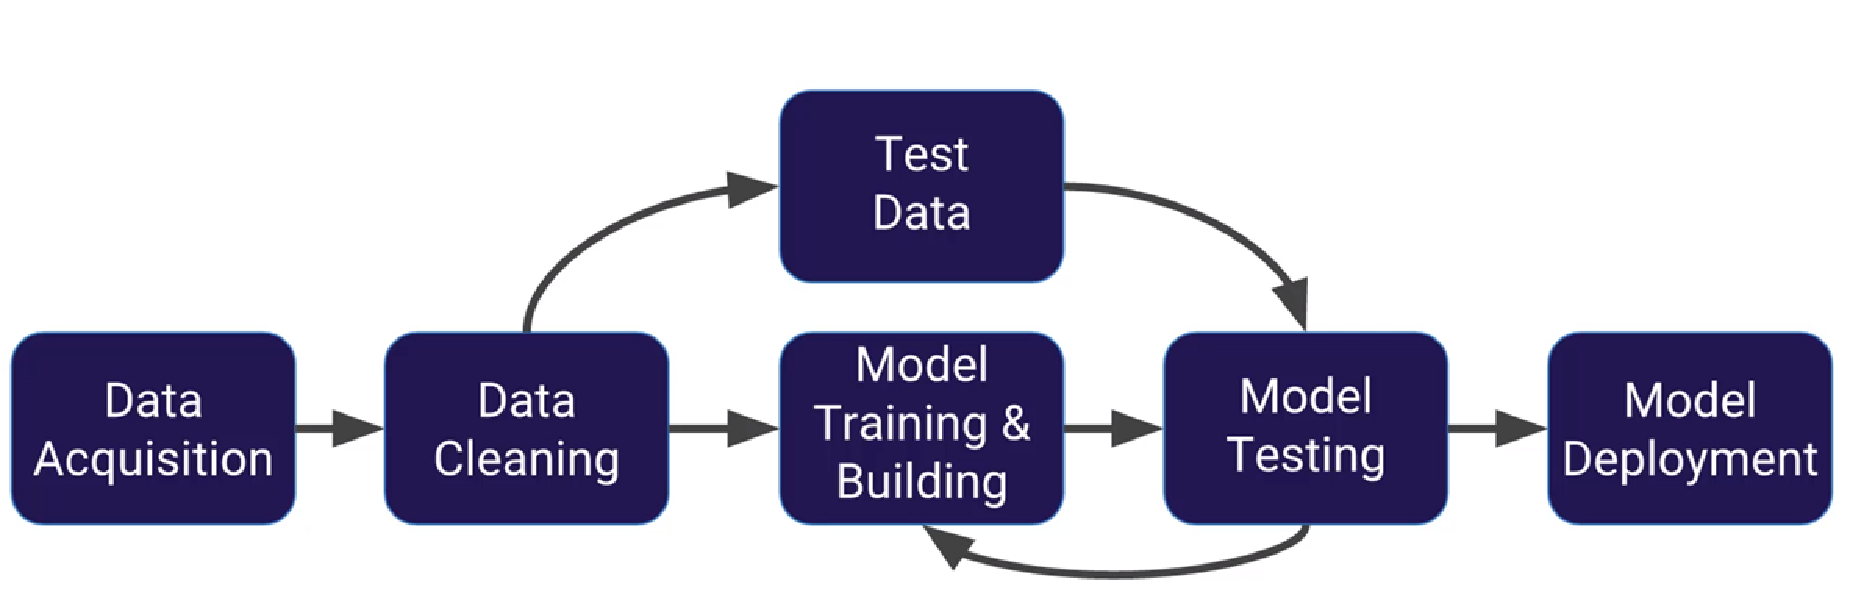
\includegraphics[scale=0.45]{./img/ml_process.pdf}
    \caption{Añadir img con evolución de las métricas dependiendo de los umbrales}
    \label{fig_mlp_18}
\end{figure}

% \begin{figure}[H]
%     \centering
%     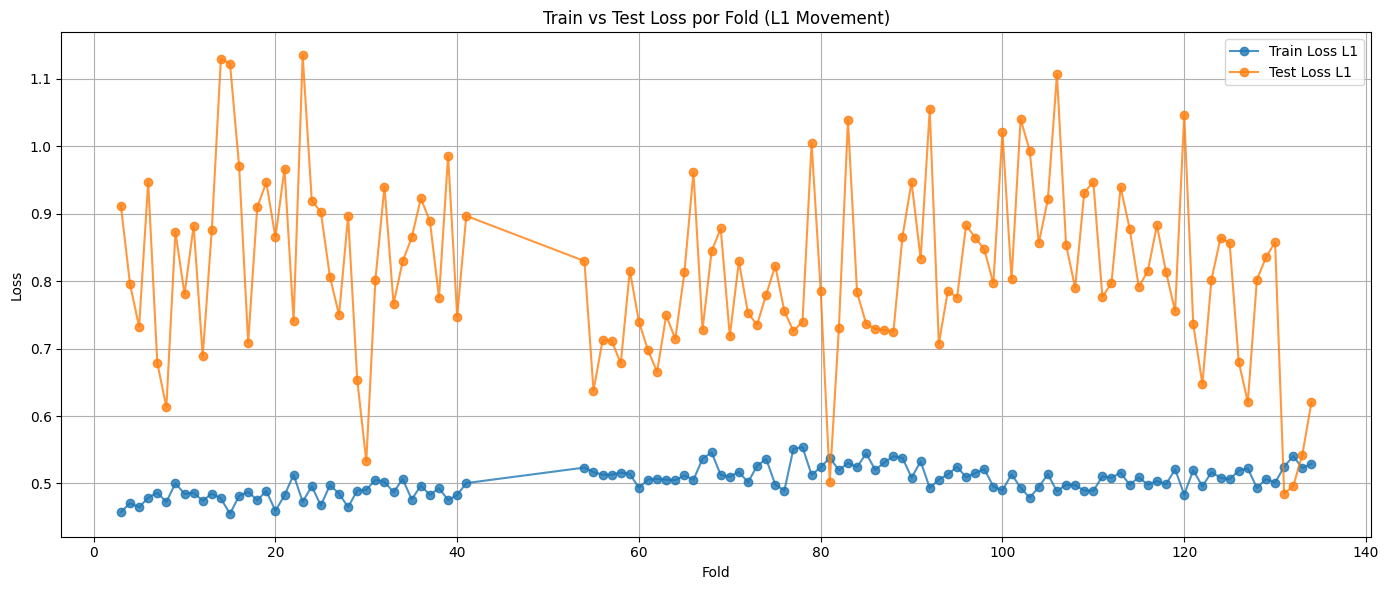
\includegraphics[width=\textwidth]{./img/loss.png}
%     \caption{Evolución de la función de pérdida en la última época de cada fold}
%     \label{fig_mlp_21}
% \end{figure}

\begin{figure}[h]
    \centering
    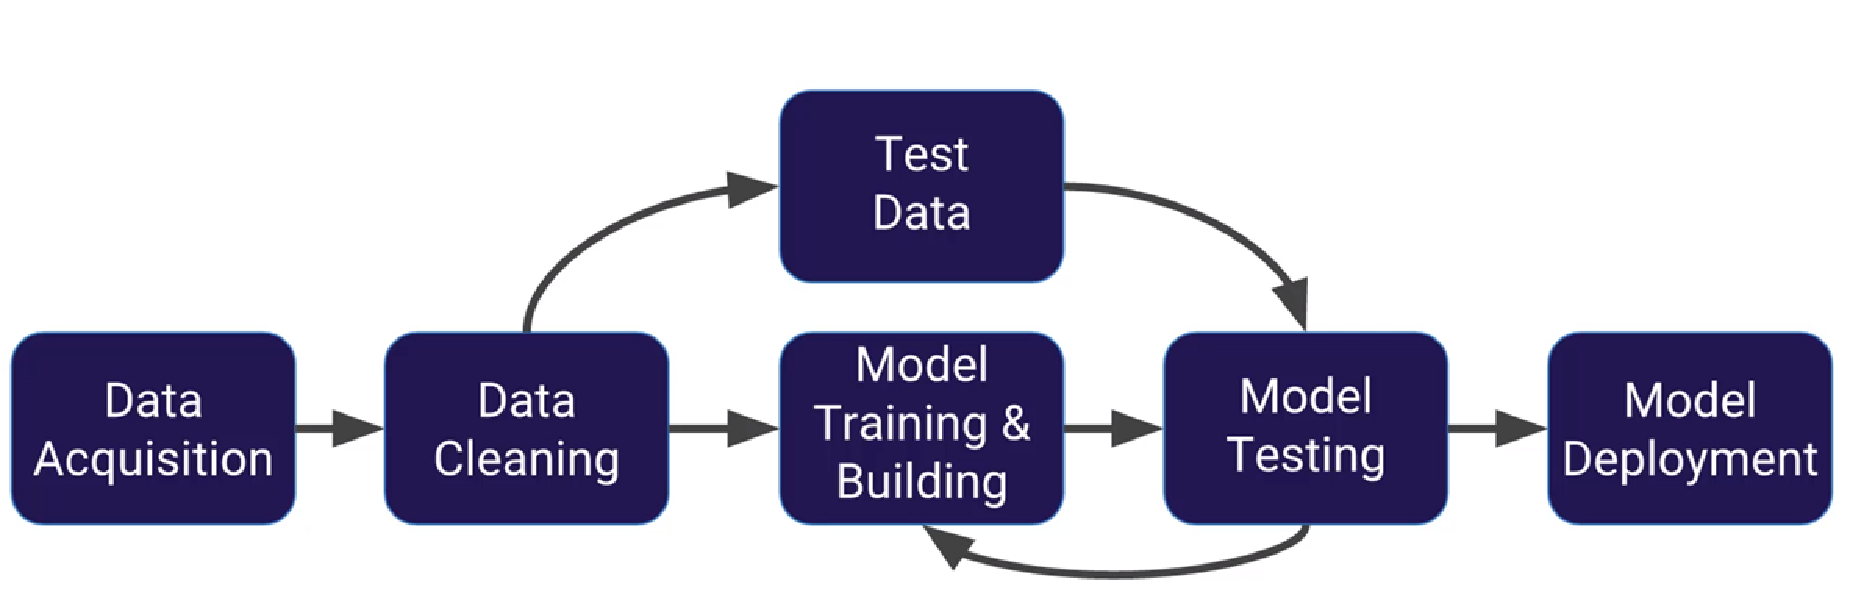
\includegraphics[scale=0.45]{./img/ml_process.pdf}
    \caption{Añadir img con una simulación de Monte Carlo con los percentiles}
    \label{fig_mlp_19}
\end{figure}

\subsection{Análisis de resultados de optimización, Backtest de la cartera y Simulación de Monte Carlo}

Una vez obtenidas las señales optimizadas para cada futuro, se realiza un análisis conjunto del comportamiento de la cartera completa. El objetivo es evaluar si la combinación de activos mejora el rendimiento respecto a operar únicamente un activo individual, así como estudiar la robustez del sistema bajo diferentes secuencias de resultados.

Para ello se lleva a cabo un nuevo backtest a nivel de cartera. En este proceso se cargan todos los \textit{trades} generados por cada futuro utilizando la estrategia operativa óptima obtenida previamente. A continuación, se construye un único \textit{DataFrame} que agrupa todas las operaciones por fecha, lo que permite simular la evolución conjunta del capital.

La simulación se realiza sobre una cuenta con un capital inicial de 1\,000\,000 USD, lo que permite incorporar restricciones realistas de riesgo y liquidez. En particular, se tienen en cuenta:

\begin{itemize}
    \item los márgenes iniciales y de mantenimiento de cada futuro,
    \item el valor nocional de cada contrato,
    \item el porcentaje máximo de capital que puede arriesgarse por operación,
    \item la exposición total máxima permitida, fijada en un 25\% del capital inicial.
\end{itemize}

Las predicciones se ordenan por nivel de confianza total y se procesan secuencialmente, verificando en cada caso que la operación no exceda los límites de margen ni las restricciones de exposición. Solo las operaciones que cumplen estas condiciones se ejecutan en la simulación.

Además del backtest, se realiza una simulación de Monte Carlo adicional para evaluar la dispersión de las métricas de la cartera completa. Para ello se agrupan los PnL diarios de todos los activos y se aplica un \textit{overlapping block bootstrap}, remuestreando bloques solapados de la serie diaria de beneficios. Este enfoque permite preservar parte de la estructura temporal y generar múltiples trayectorias alternativas del rendimiento de la cartera.

El análisis conjunto del backtest y de la simulación de Monte Carlo permite comparar el rendimiento de la cartera diversificada frente a la operativa de un único activo, así como evaluar la estabilidad del sistema bajo diferentes escenarios de mercado.
